
%(BEGIN_QUESTION)
% Copyright 2011, Tony R. Kuphaldt, released under the Creative Commons Attribution License (v 1.0)
% This means you may do almost anything with this work of mine, so long as you give me proper credit

Skriv en ligning for å beregne nedstrøms trykk i denne reguleringsventilen, gitt oppstrøms trykk ($P_1$), $C_v$-faktor, spesifikk vekt ($G_f$) for prosessvæsken og strømningsrate ($Q$):

$$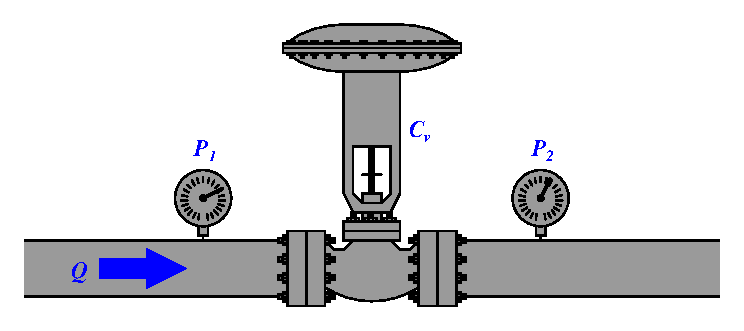
\includegraphics[width=15.5cm]{i01501x01.eps}$$

\vskip 10pt

$P_2$ (formel) = 

\vskip 20pt

Beregn deretter $P_2$ (i PSI) med følgende betingelser:

\begin{itemize}
\item{} $Q$ = 130 GPM
\item{} $G_f$ = 0.83
\item{} $P_1$ = 260 kPa
\item{} $C_v$ = 35
\end{itemize}

\vskip 10pt

$P_2$ = \underbar{\hskip 50pt} PSI

\underbar{file i01501}
%(END_QUESTION)





%(BEGIN_ANSWER)

Halv uttelling for korrekt formel, halv uttelling for korrekt tallsvar:

\vskip 10pt

$$P_2 = P_1 - G_f \left( {Q \over C_v} \right)^2$$

\vskip 10pt

$P_2$ = 26.26 PSI

%(END_ANSWER)





%(BEGIN_NOTES)

{\bf Denne oppgaven er ment for prøver/eksamen, ikke arbeidsark!}

%(END_NOTES)

